% Please make sure you insert your
% data according to the instructions in PoSauthmanual.pdf
\documentclass[a4paper,11pt]{article}
\usepackage{pos}

\usepackage{caption}
\usepackage{float}
\usepackage[lofdepth=1,lotdepth]{subfig}

\usepackage[noabbrev, capitalise, nameinlink]{cleveref}  % reference object types automatically

\title{Search for heavy neutral lepton production and decay with the IceCube Neutrino Observatory}
%% \ShortTitle{Short Title for header}

\author*[a]{Leander Fischer}
\author[b]{Julia Book}


\affiliation[a]{DESY, D-15738 Zeuthen, Germany}
\affiliation[b]{Harvard University, Cambridge, MA 02138, USA}

\emailAdd{leander.fischer@desy.de}
\emailAdd{jbook@g.harvard.edu}

\abstract{ Searching for HNLs with IceCube is soooooo much fun.. }

\FullConference{%
  41st International Conference on High Energy physics - ICHEP2022\\
  6-13 July, 2022\\
  Bologna, Italy
}

%% \tableofcontents

\begin{document}
\maketitle


\section{Introduction}

\begin{itemize}
  \item Motivate the search for (heavy) sterile neutrinos
  \item Cite the relevant papers
  % \item 
\end{itemize}


\begin{figure}
  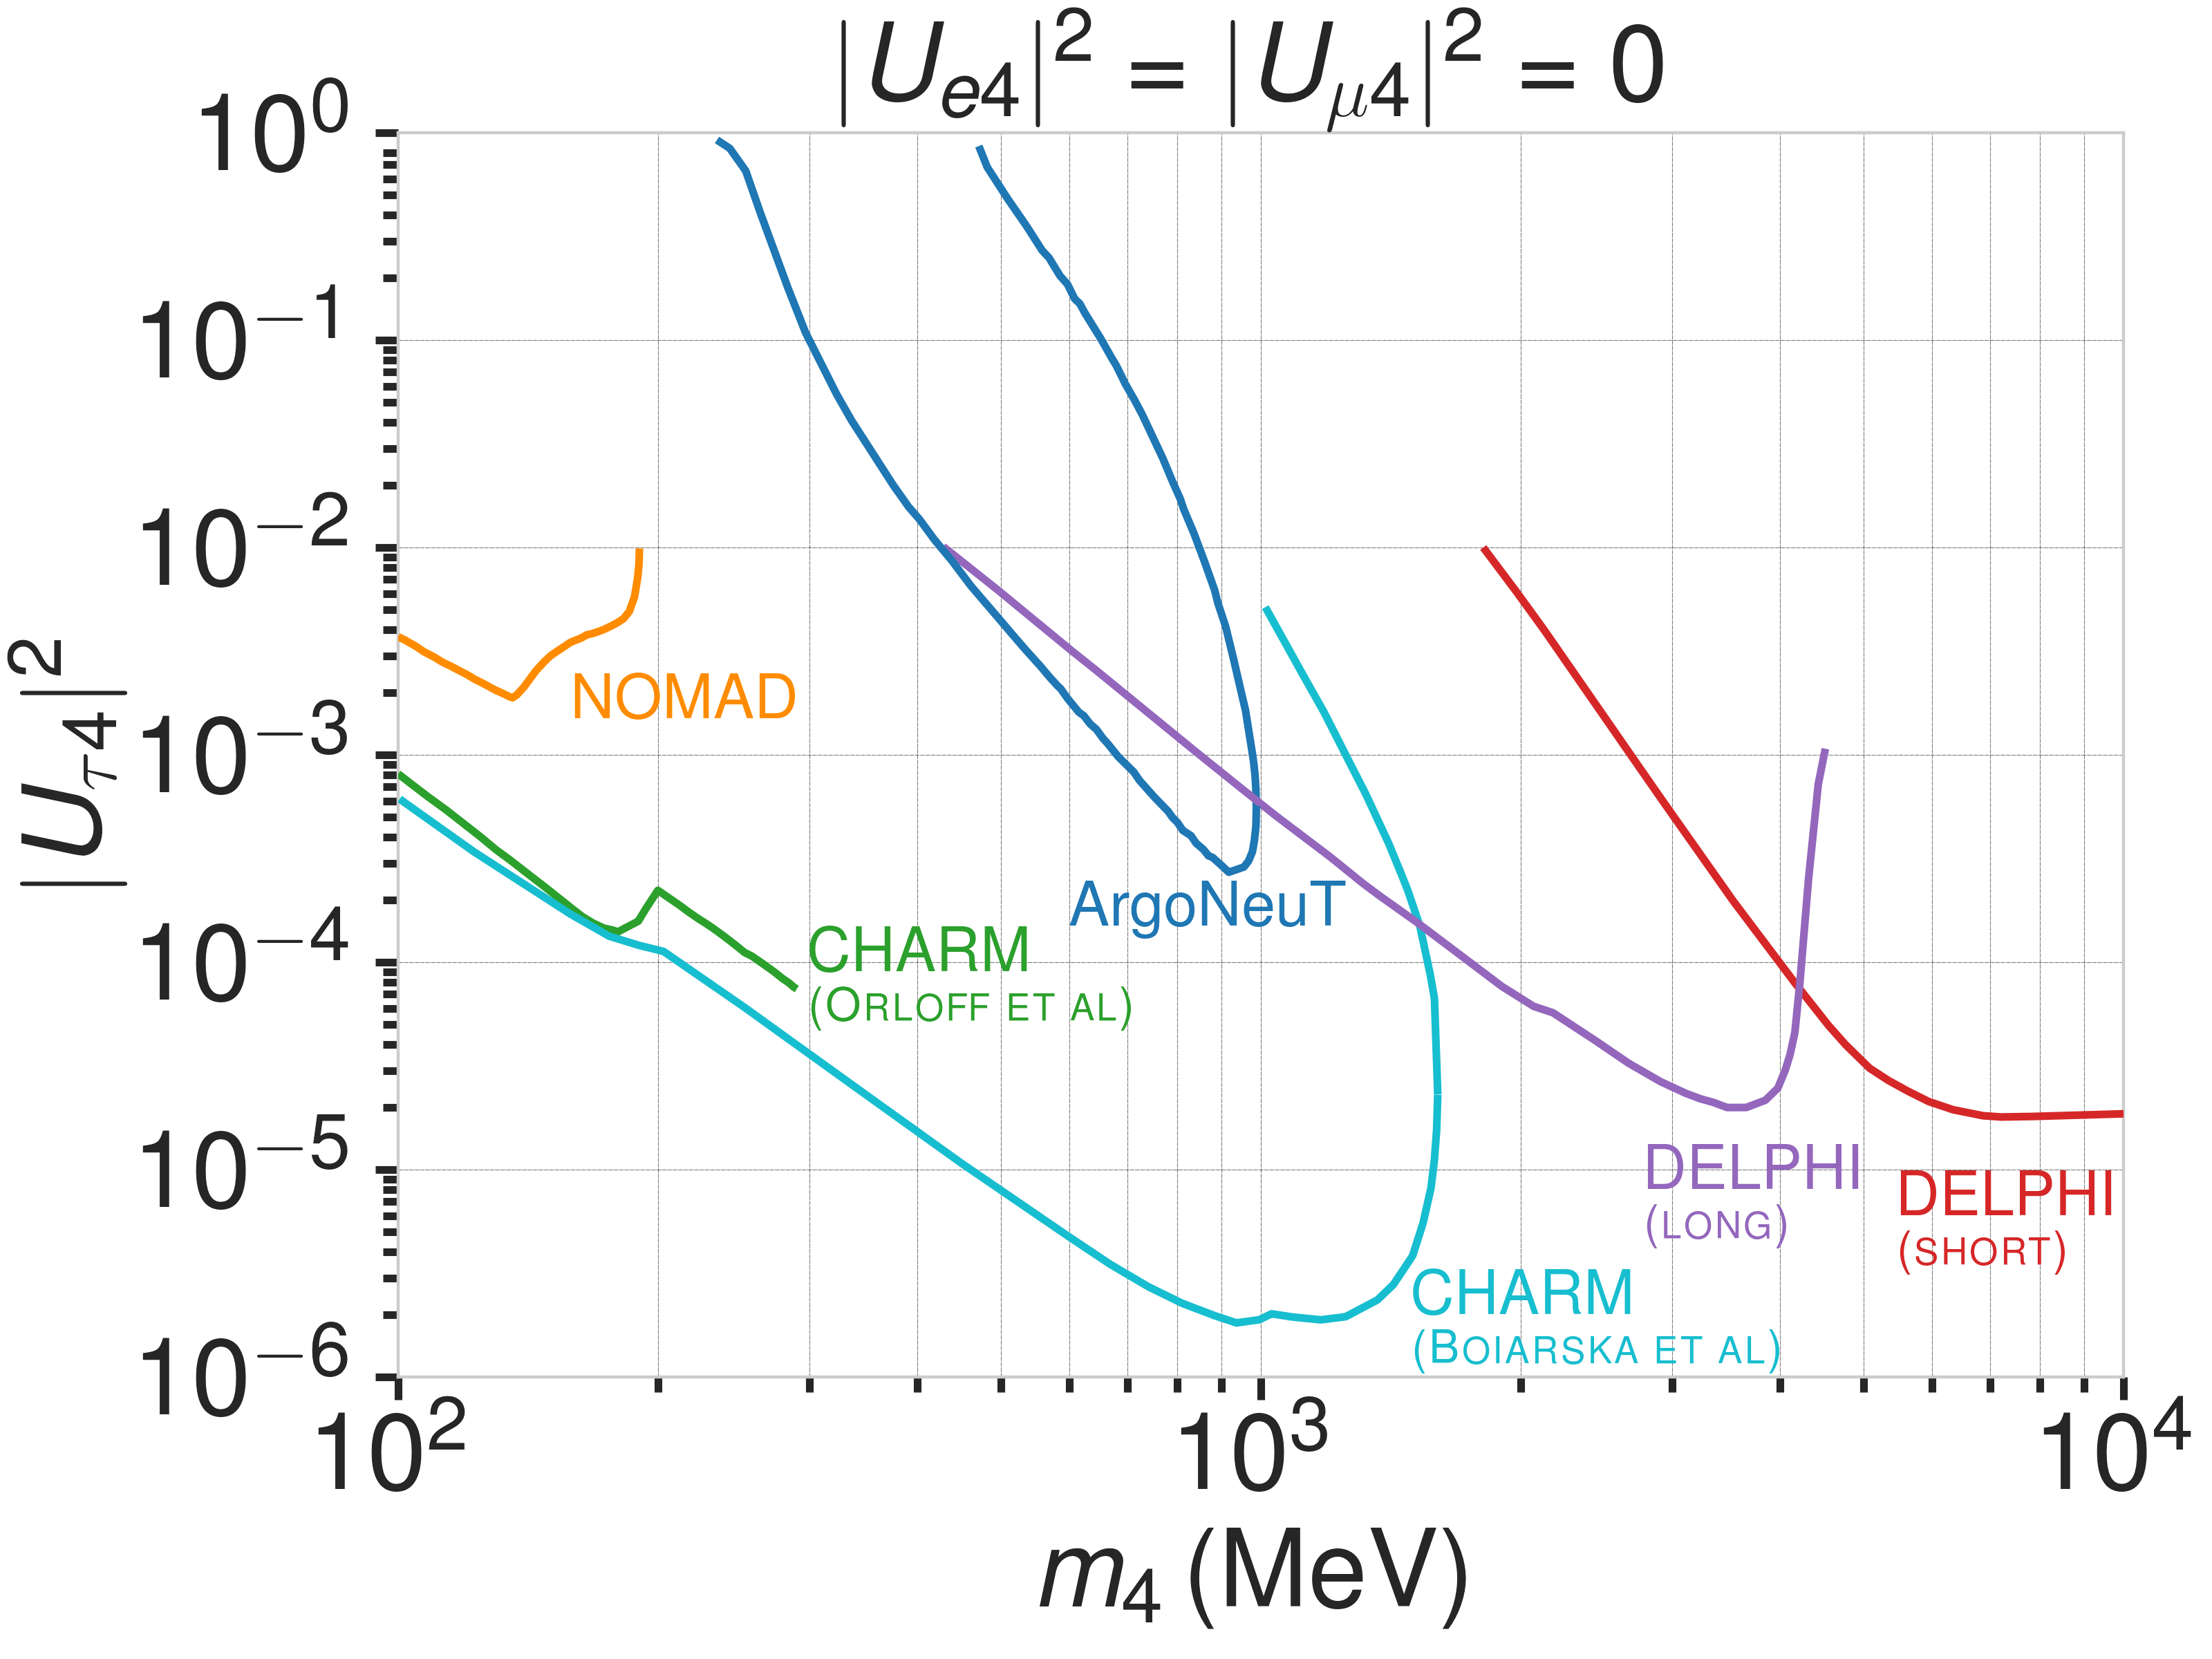
\includegraphics[width=.50\linewidth]{figures/UtauN_custom_plots_LF_grid_white.png}
  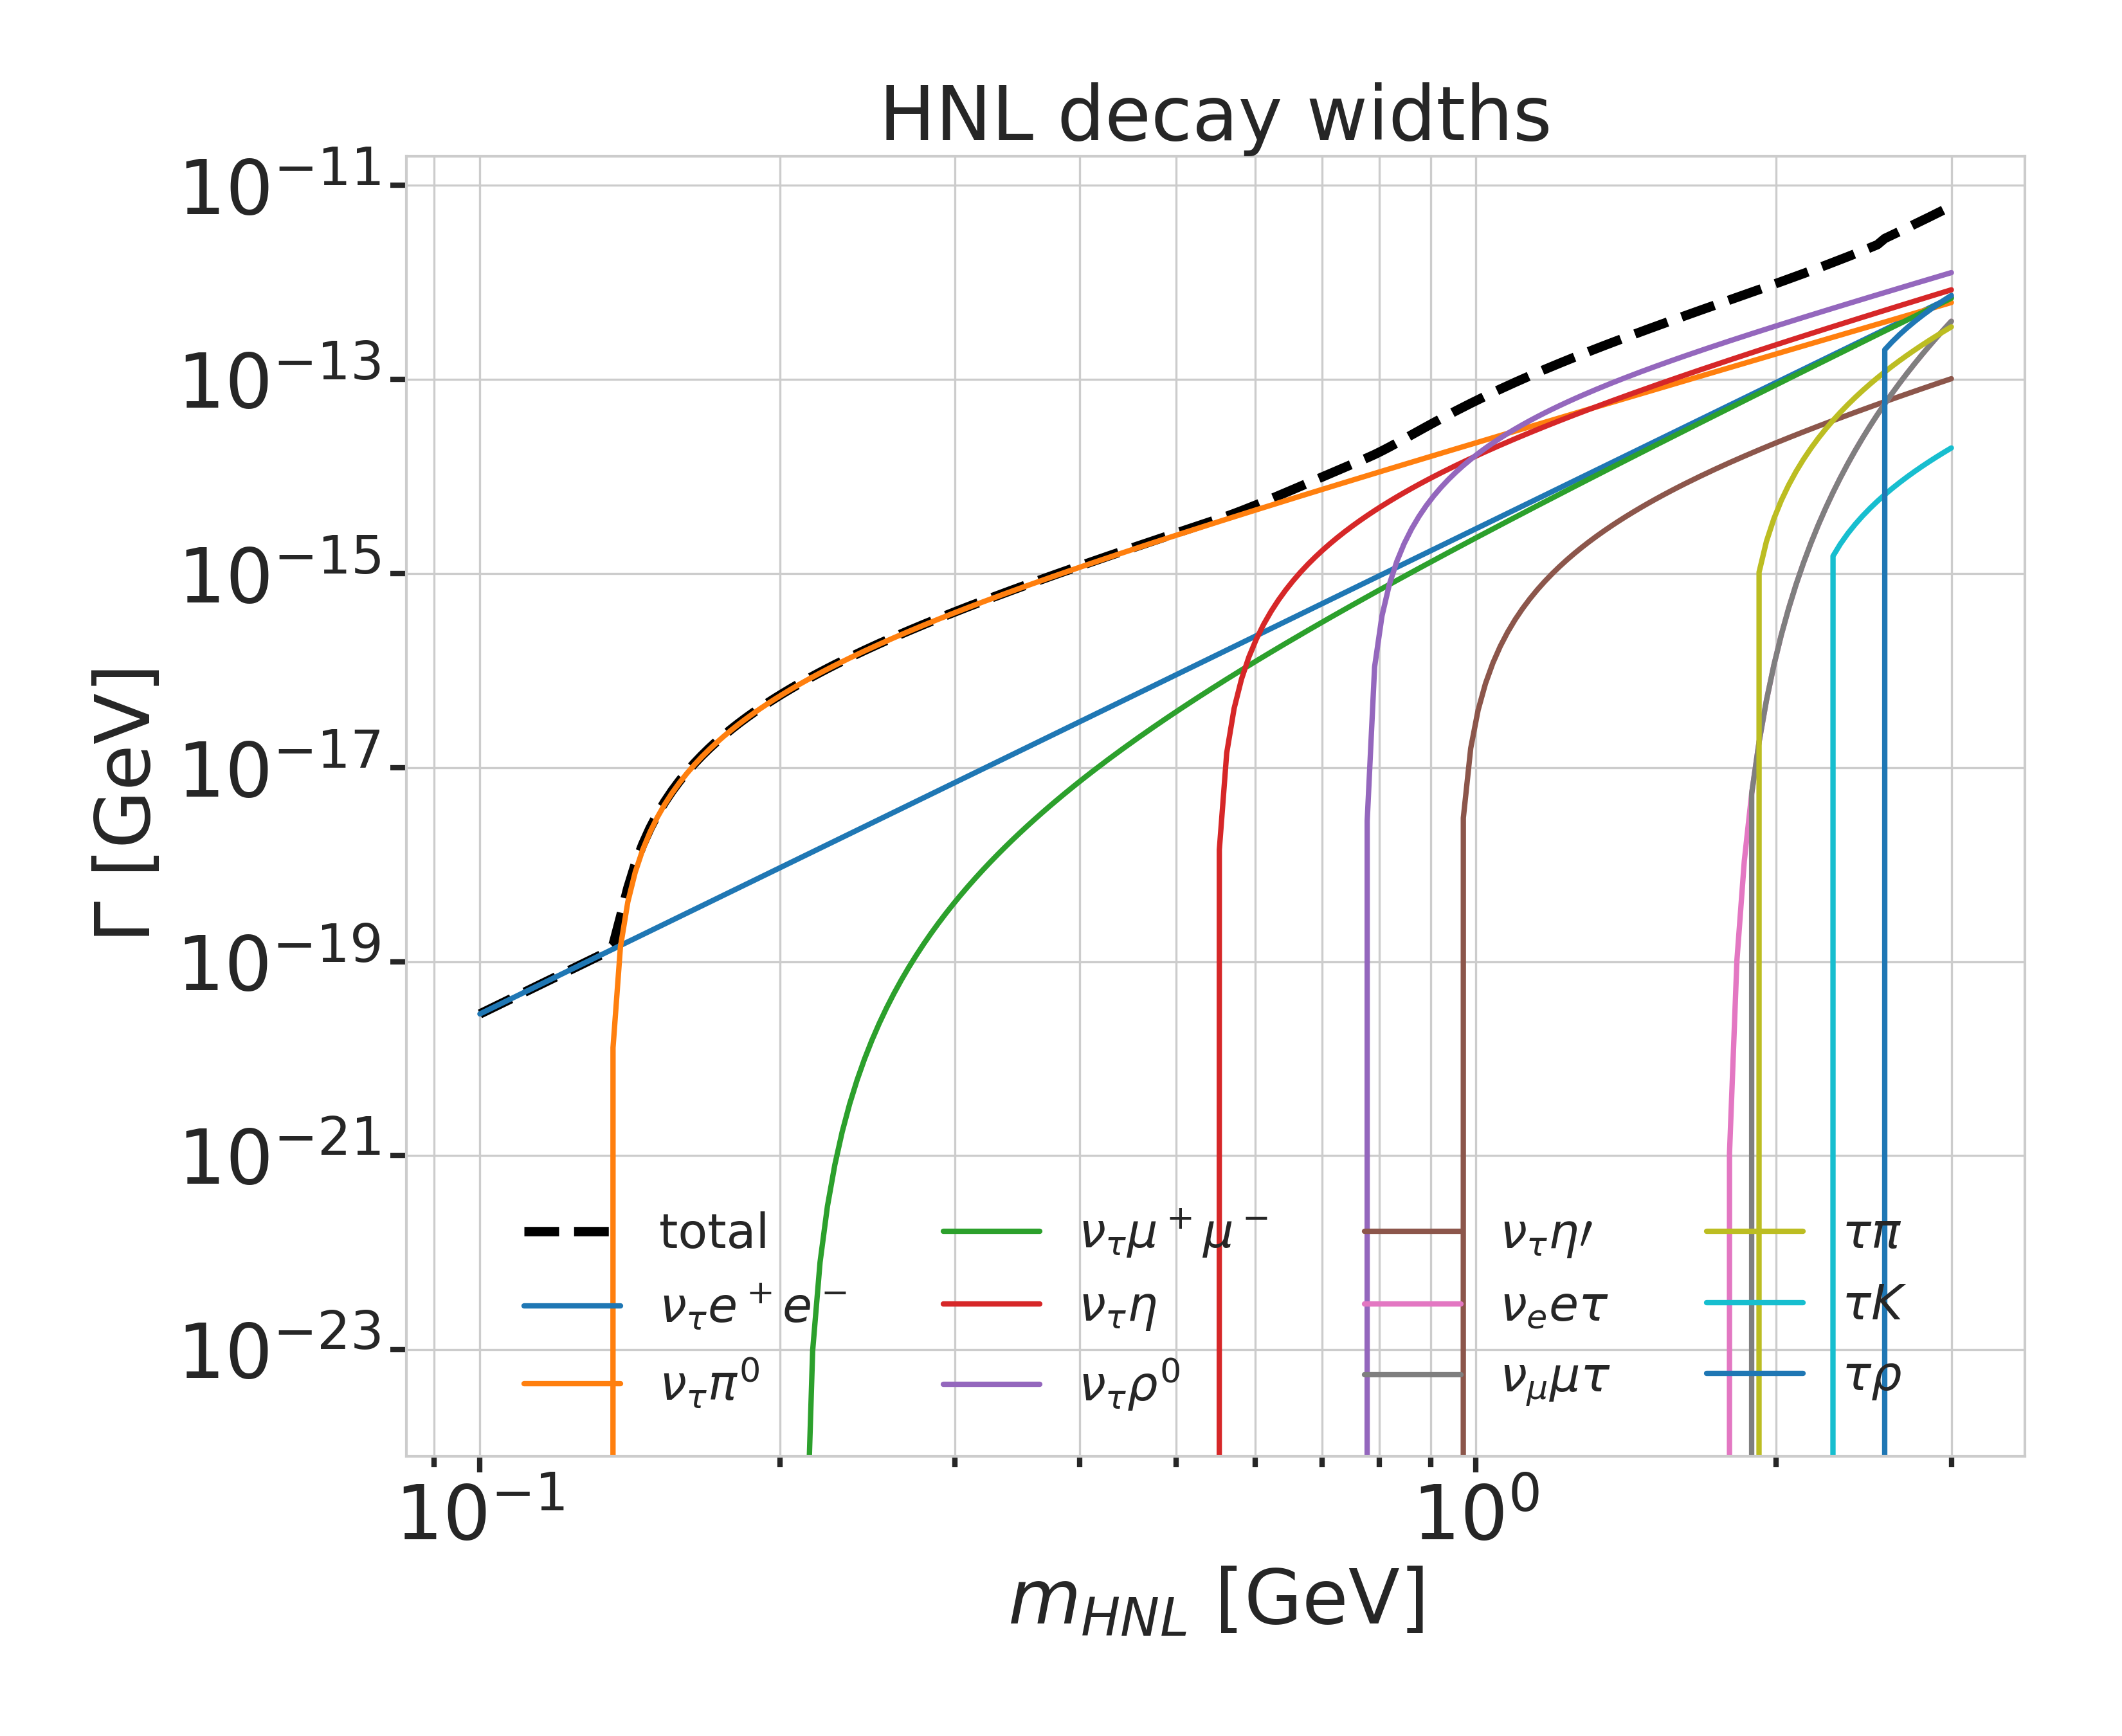
\includegraphics[width=.47\linewidth]{figures/hnl_decay_widths_log.png}
  \label{fig:hnl_visible_decay_widths}
  \caption{Current $|U_{\tau4}^2|$ limits (left) from NOMAD \cite{NOMAD:2001eyx}, ArgoNeut \cite{ArgoNeuT:2021clc}, CHARM \cite{Orloff:2002de, Boiarska:2021yho}, and DELPHI \cite{DELPHI:1996qcc} and decay widths of visible decay modes in IceCube (right) calculated based on the results from \cite{Gorbunov:2007ak}.}
  \label{fig:hnl_limits_and_decay_widths}
\end{figure}


\section{IceCube DeepCore}

The IceCube Neutrino Observatory \cite{Aartsen:2016nxy} is located at the geographic South Pole and consists of 5160 Digital Optical Modules (DOMs), deployed into the antarctic glacial ice at depths between 1.45\,km and 2.45\,km. It is an ice Cherenkov telescope instrumenting a volume of about 1\,km$^{3}$. The ice is used as interaction and detection medium, simultaneously, where interacting neutrinos can produce charged secondary particles, which themselves can emit Cherenkov photons detectable by the DOMs. The DOMs are arranged on a nearly-hexagonal array, as shown in \cref{fig:icecube_array}, with 125\,m horizontal and 17\,m vertical spacing in IceCube and a closer 42-72\,m horizontal of 7\,m vertical spacing in the denser, bottom-center part of the array, called DeepCore \cite{IceCube:2011ucd}. While IceCube targets the detection of astrophysical neutrinos with energies above $\sim$100\,GeV, DeepCore can measure neutrino interactions down to a few GeV, due to its closer spacing in regions with very good optical properties of the ice. This allows the measurement of atmospheric neutrino oscillations that occur mainly occur in the 10-50\,GeV region. The location of DeepCore is also indicated in \cref{fig:icecube_array}, which also shows the absorption properties of the ice with respect to depth.

\begin{figure}[h]
  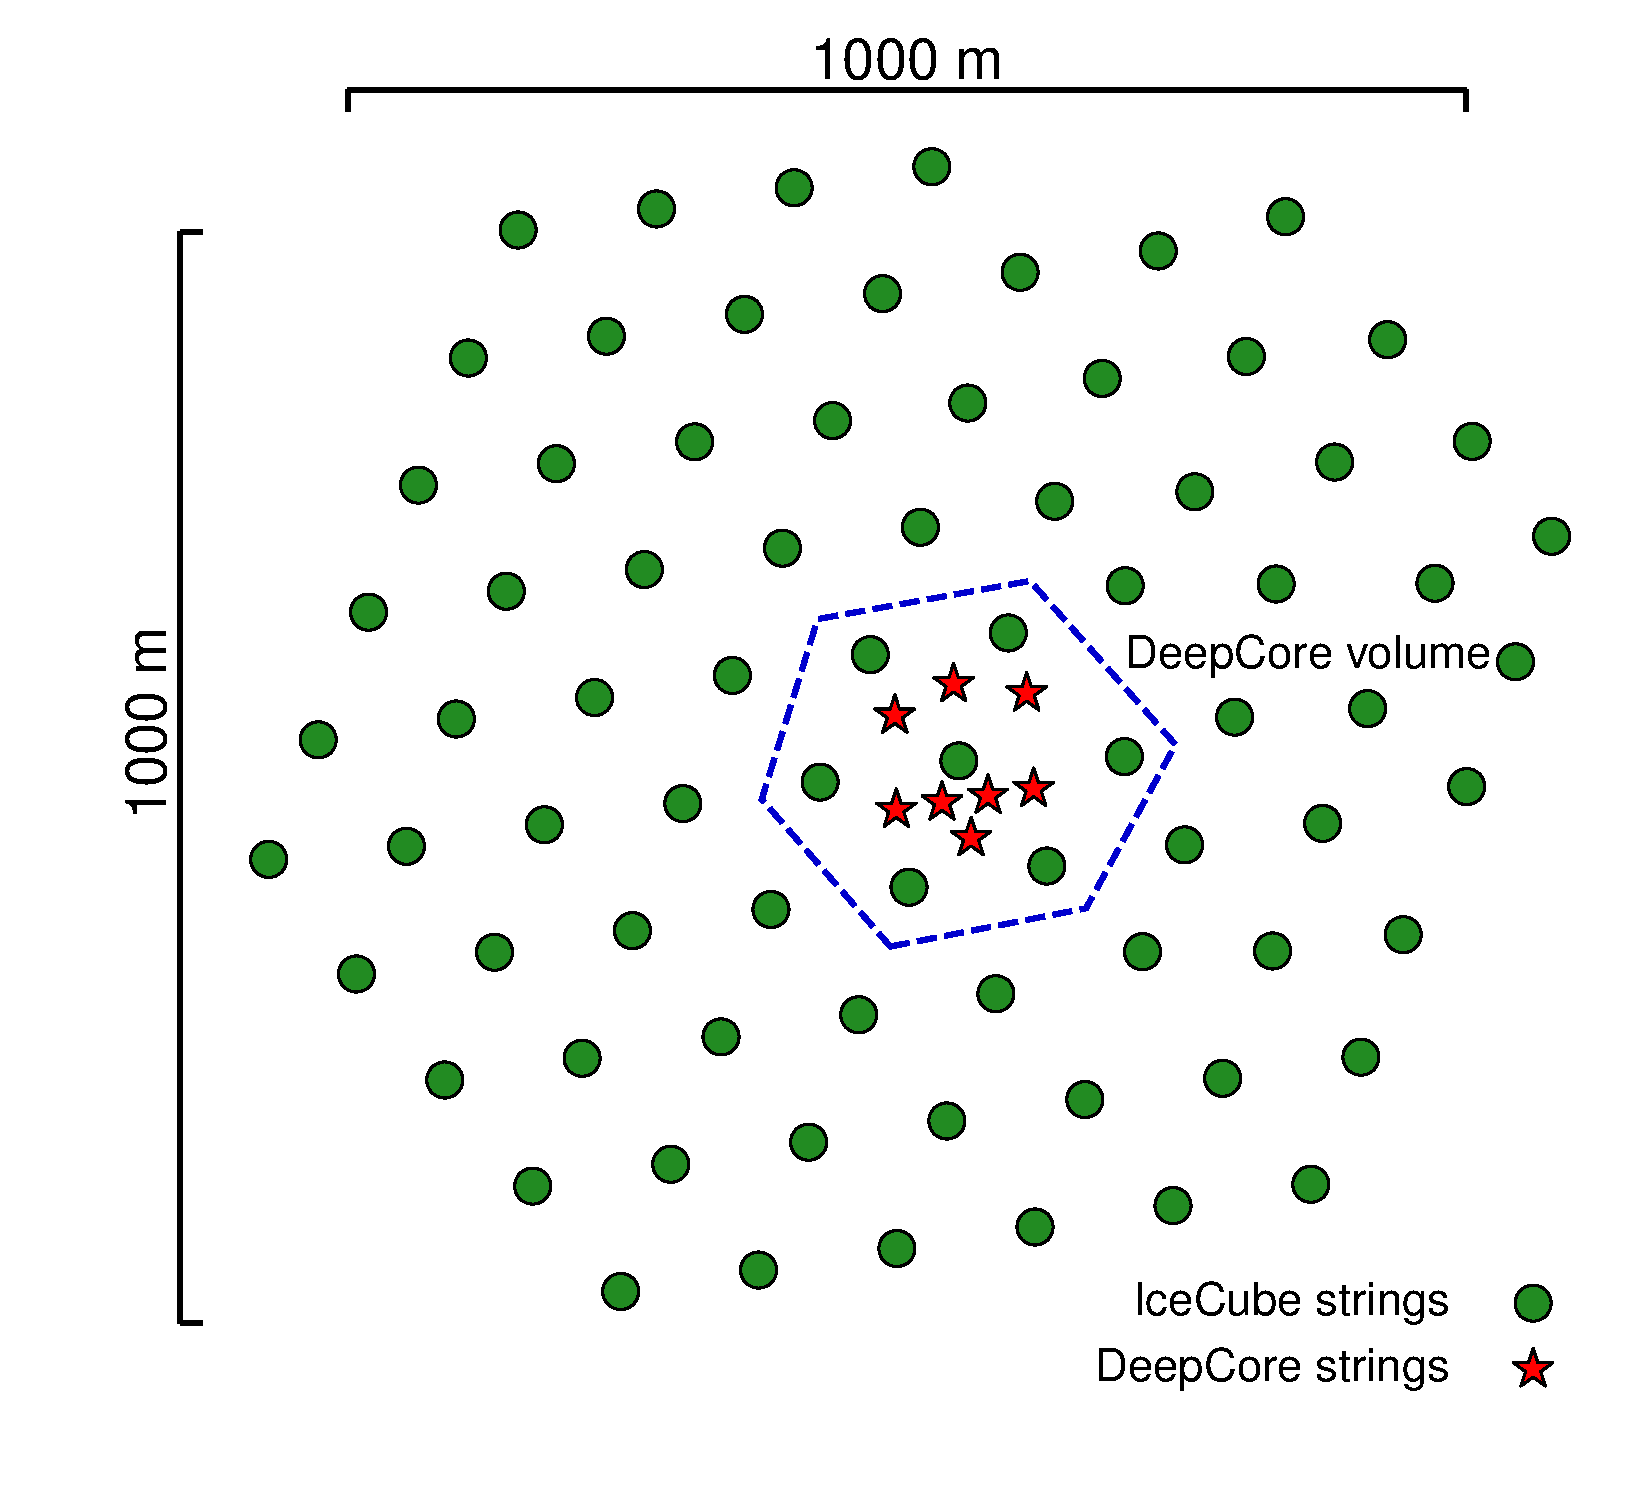
\includegraphics[width=.43\linewidth]{figures/icecube_top_view_bw.pdf}
  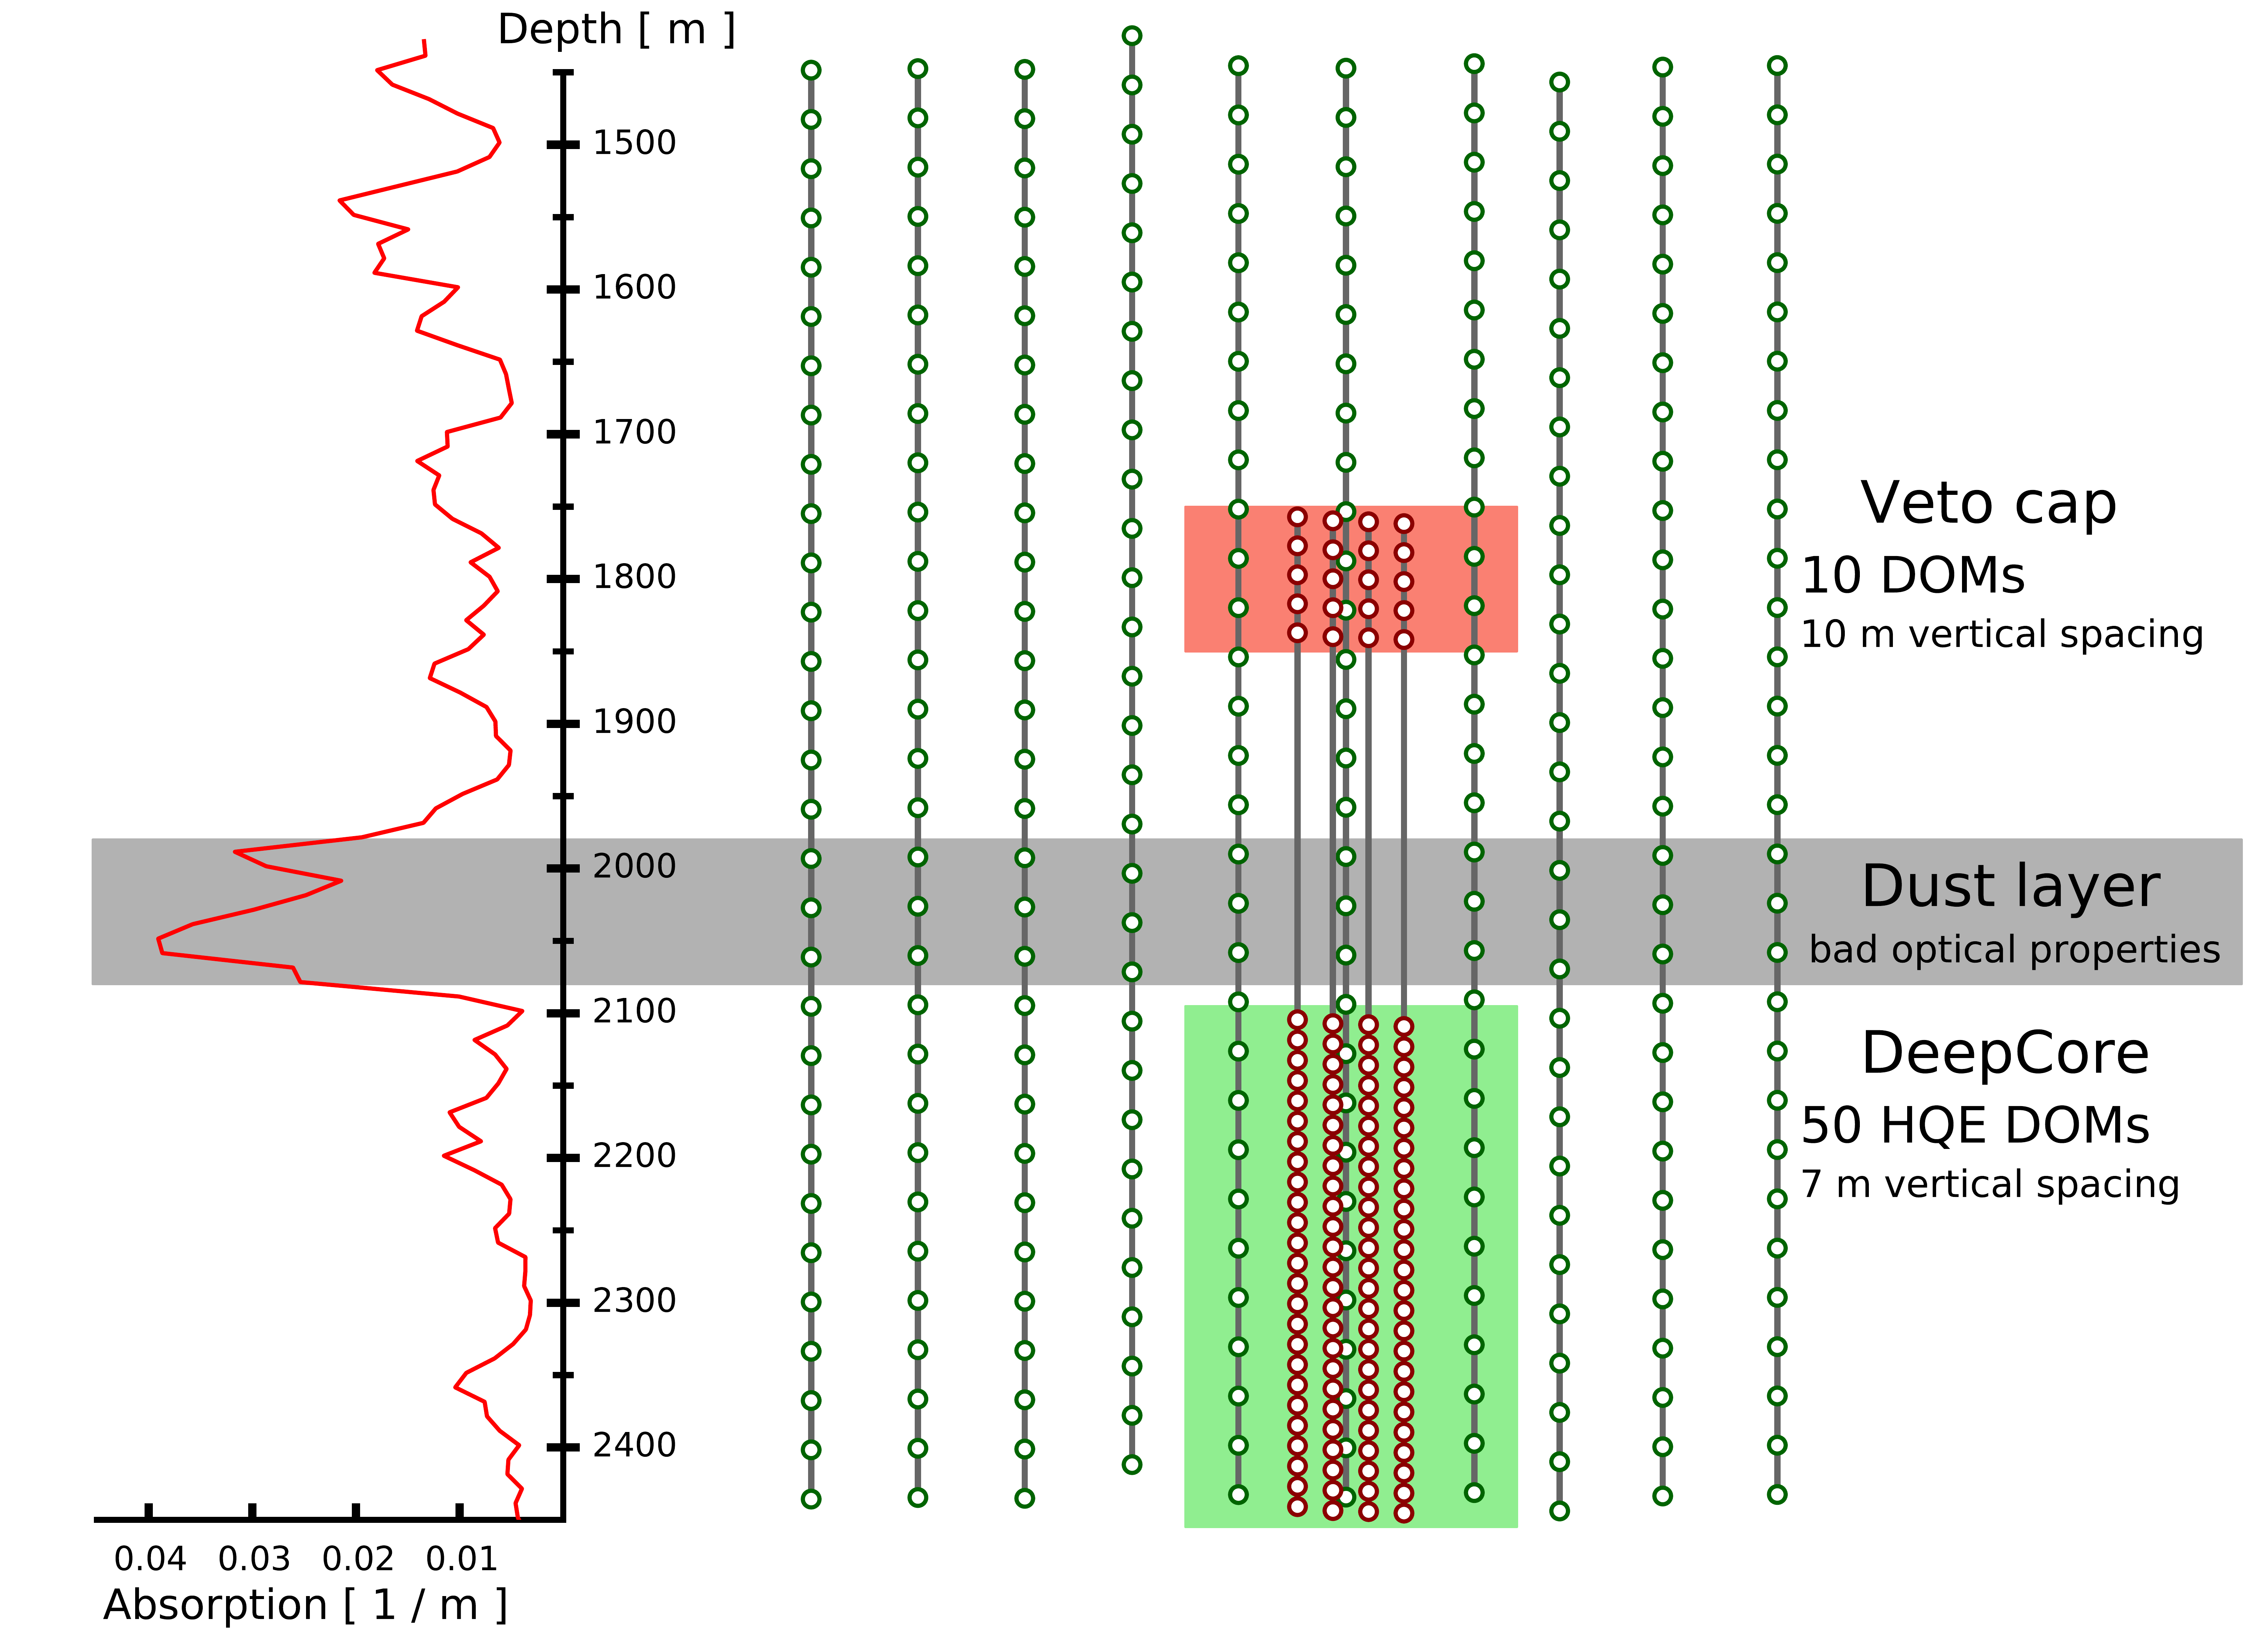
\includegraphics[width=.52\linewidth]{figures/DeepCore_sideview.png}
  \caption{Top (left) and side (right) view of the IceCube and DeepCore array. The side view also shows the ice absorption at different depths.}
  \label{fig:icecube_array}
\end{figure}

The two observable, low energy event topologies in IceCube DeepCore are \textit{tracks} and \textit{cascades}. Tracks are elongated light emission patterns, produced by long-lived muons, mainly originating from $\nu_{\mu}$ CC interactions or cosmic ray air showers, with a subdominant component from $\nu_{\tau}$ CC interactions (BR of $\tau\rightarrow\mu$ $\sim 17\%$ \cite{PhysRevD.98.030001}). Cascades are roughly point-like, spherical light emissions, produced by electromagnetic and hadronic showers. They are produced by $\nu_{e}$ and most $\nu_{\tau}$ CC interactions, as well as NC interactions of all flavours.

\begin{figure}[h]
  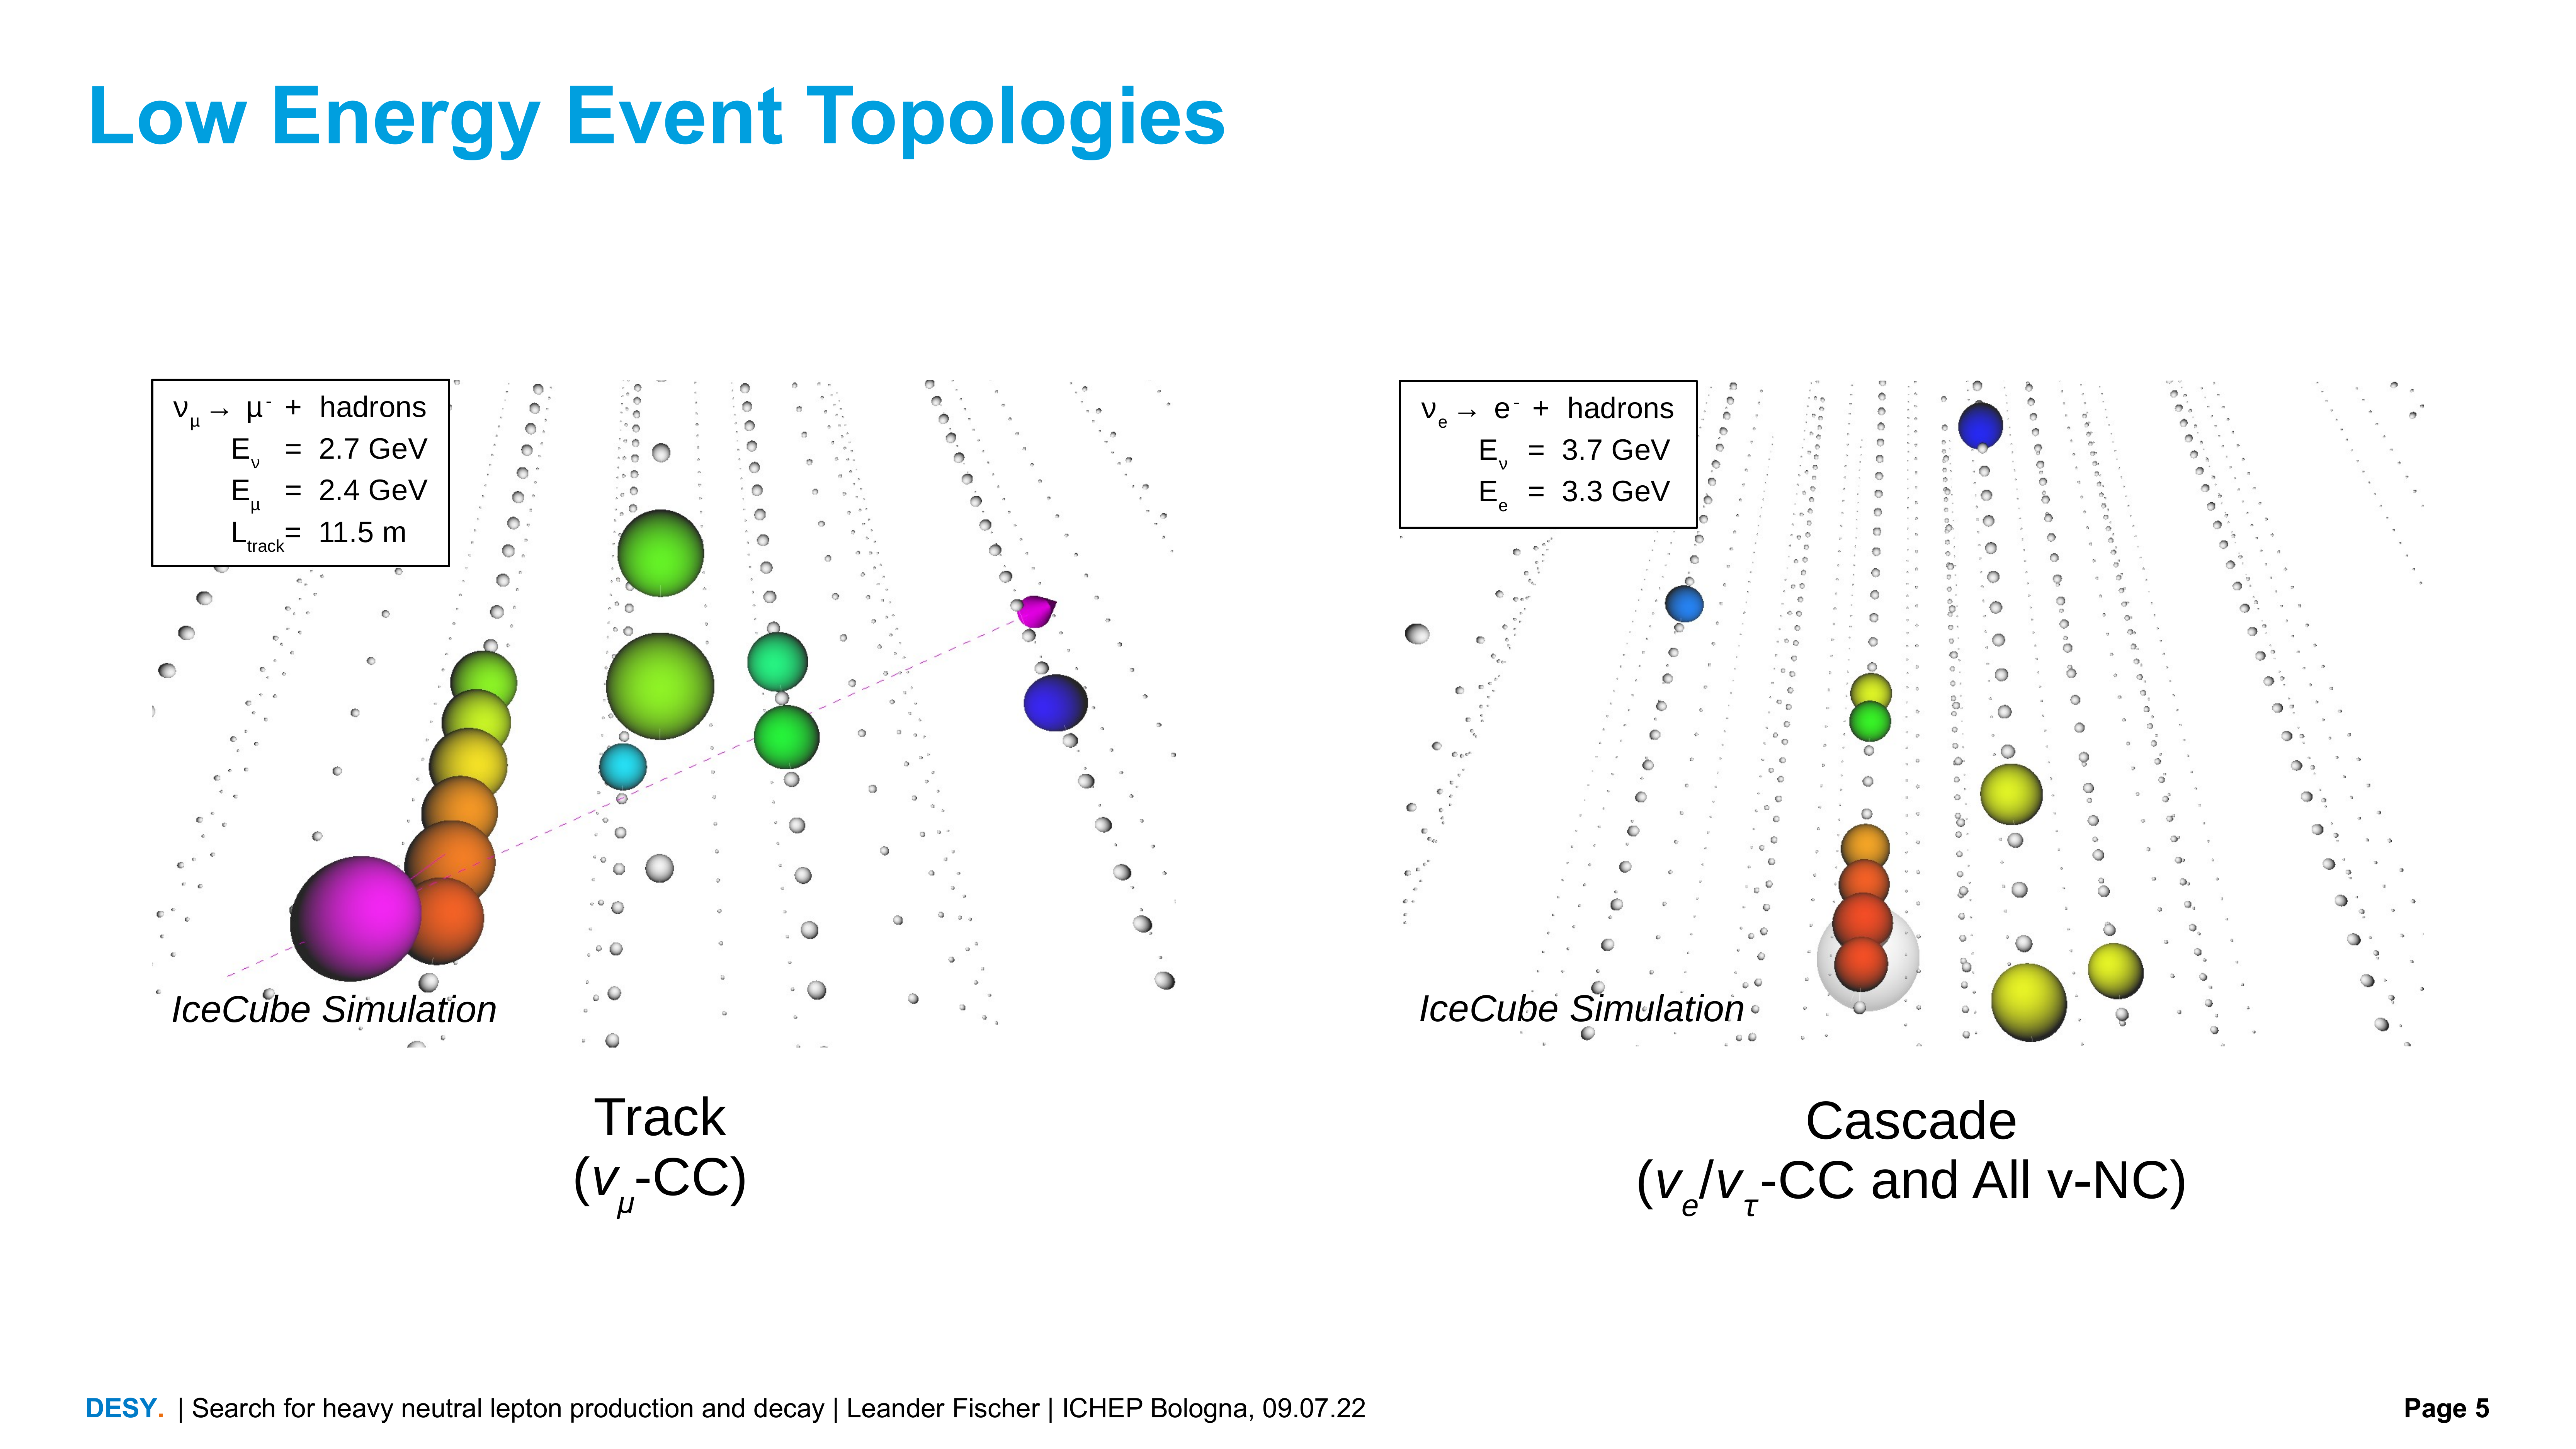
\includegraphics[trim = 2cm 3cm 2cm 5cm, clip, width=1.0\linewidth]{figures/event_views.png}
  \caption{Example of low energy event topologies in IceCube DeepCore. The color of the spheres indicates the arrival time of the photons while its size is relative to the number of photons that were detected.}
  \label{fig:low_energy_eventviews}
\end{figure}


\section{Neutrino Oscillations} \label{sec:neutrino_oscillations}

\begin{itemize}
  \item mass/flavor mixing
  \item testable phase space (ennergy/zenith)
  \item 10 year data sample + rates
  \item IC/DC oscillation results (OVS, hight stats prediction)
\end{itemize}


\section{Heavy neutral lepton search}

\begin{itemize}
  \item model details
  \item double cascade signatures (up scattering, decay (decay modes))
  \item low energy event signature (double cascade)
  \item nutau detection channel (mass-energy-mixing-decay length relation)
  \item issues/takeaways
  \item envisioned analysis principle
\end{itemize}


% \begin{figure}
%   \centering
%   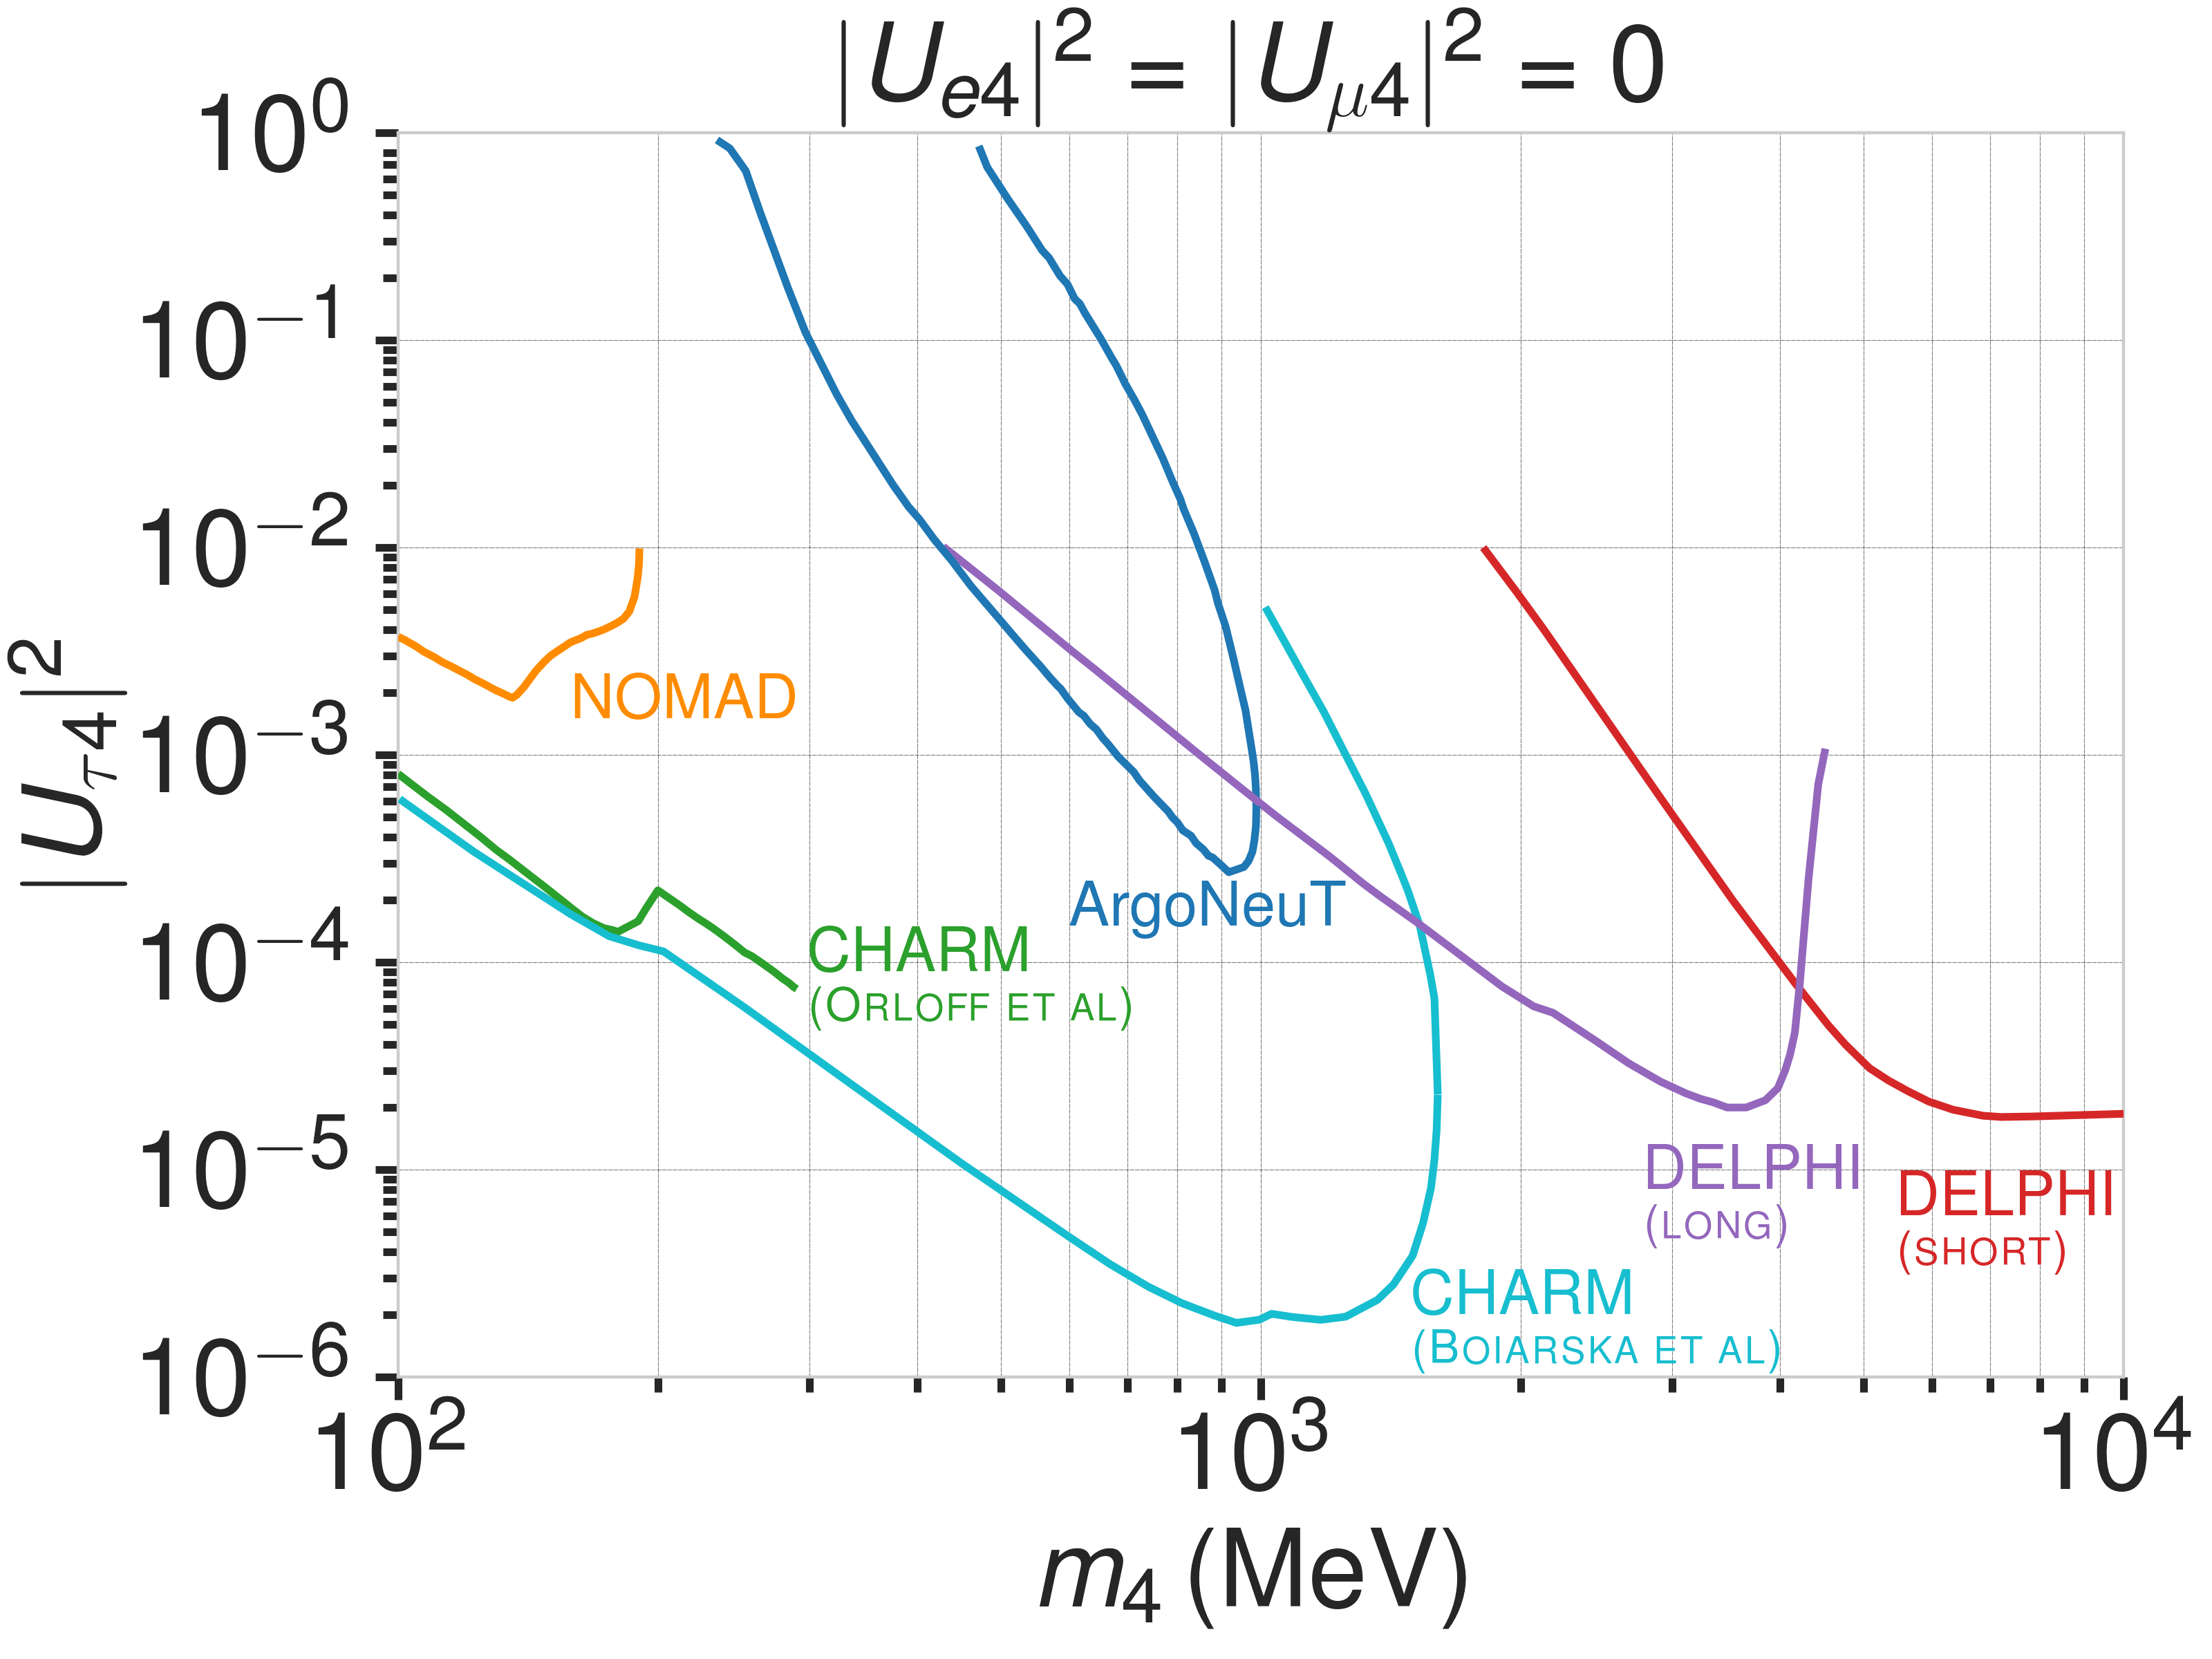
\includegraphics[width=0.49\textwidth]{figures/UtauN_custom_plots_LF_grid_white.png}
%   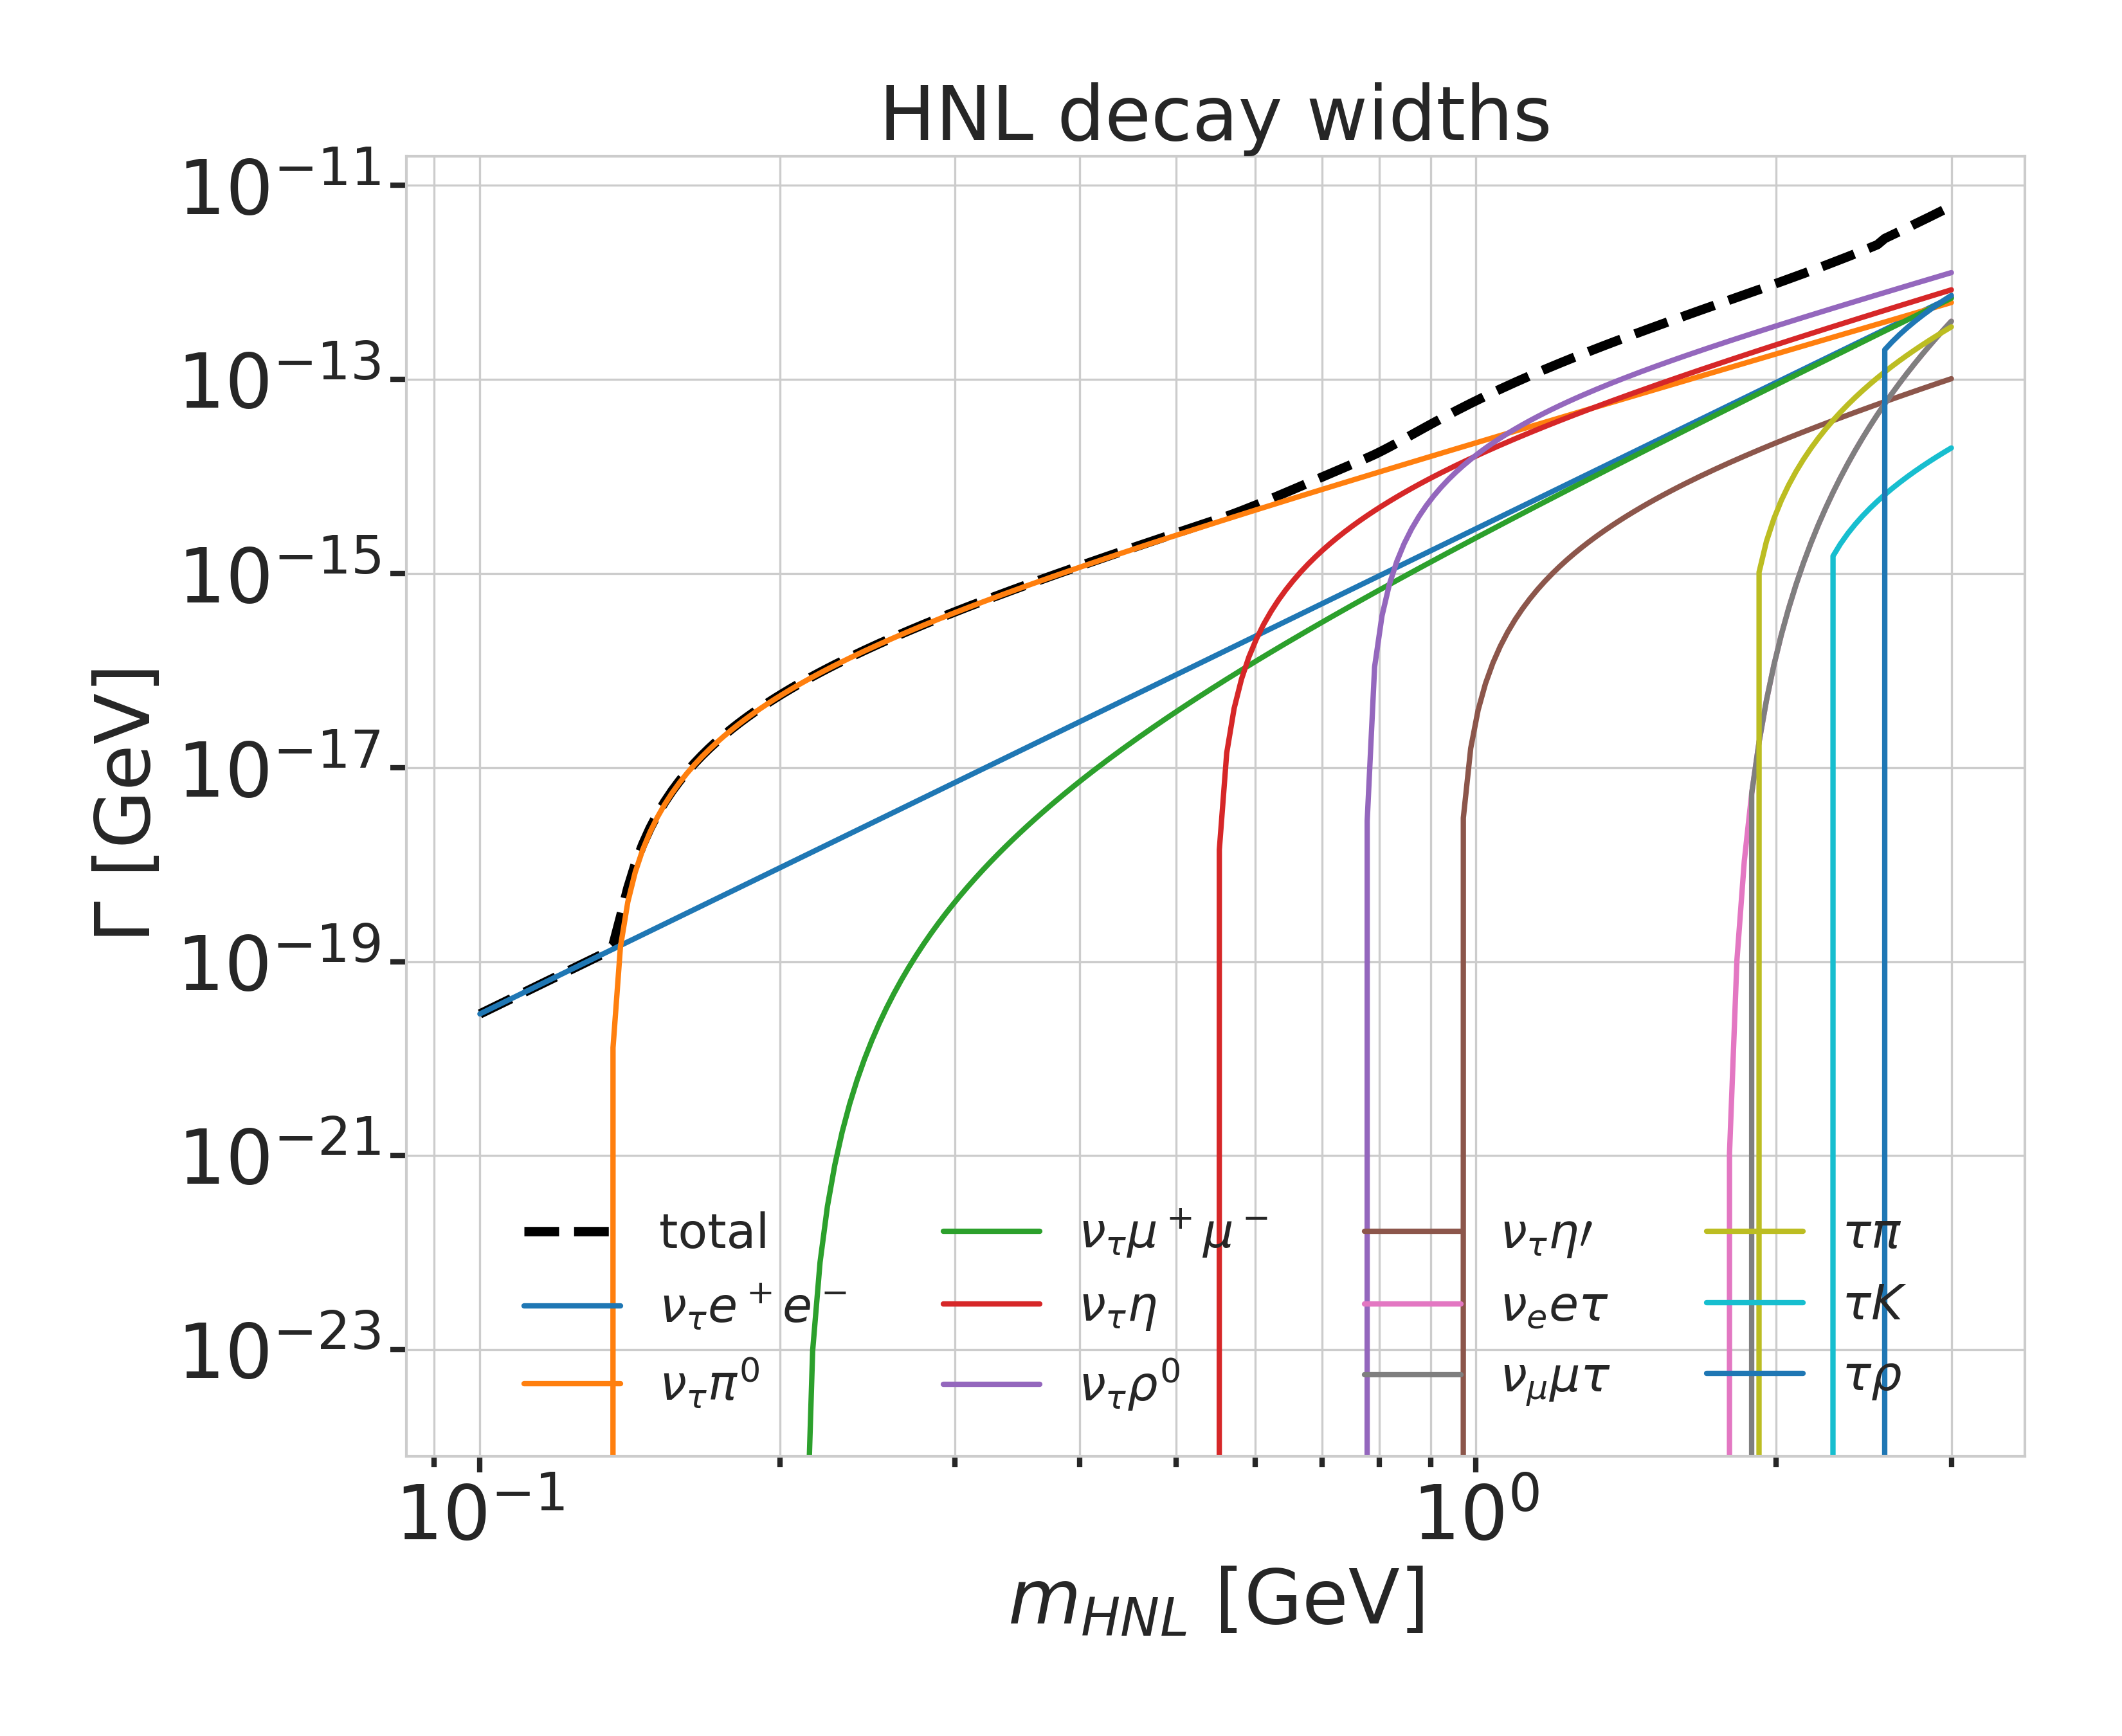
\includegraphics[width=0.49\textwidth]{figures/hnl_decay_widths_log.png}
%   \caption{Current constraints on $|U_{\tau4}^2|$ in the mass range of $[0.1,10.0]$\,GeV. Limits are from NOMAD \cite{NOMAD:2001eyx}, ArgoNeut \cite{ArgoNeuT:2021clc}, CHARM \cite{Orloff:2002de, Boiarska:2021yho}, and DELPHI \cite{DELPHI:1996qcc}.}
%   \label{fig:boundsUtau}
% \end{figure}


% \begin{figure}
%   \centering
%   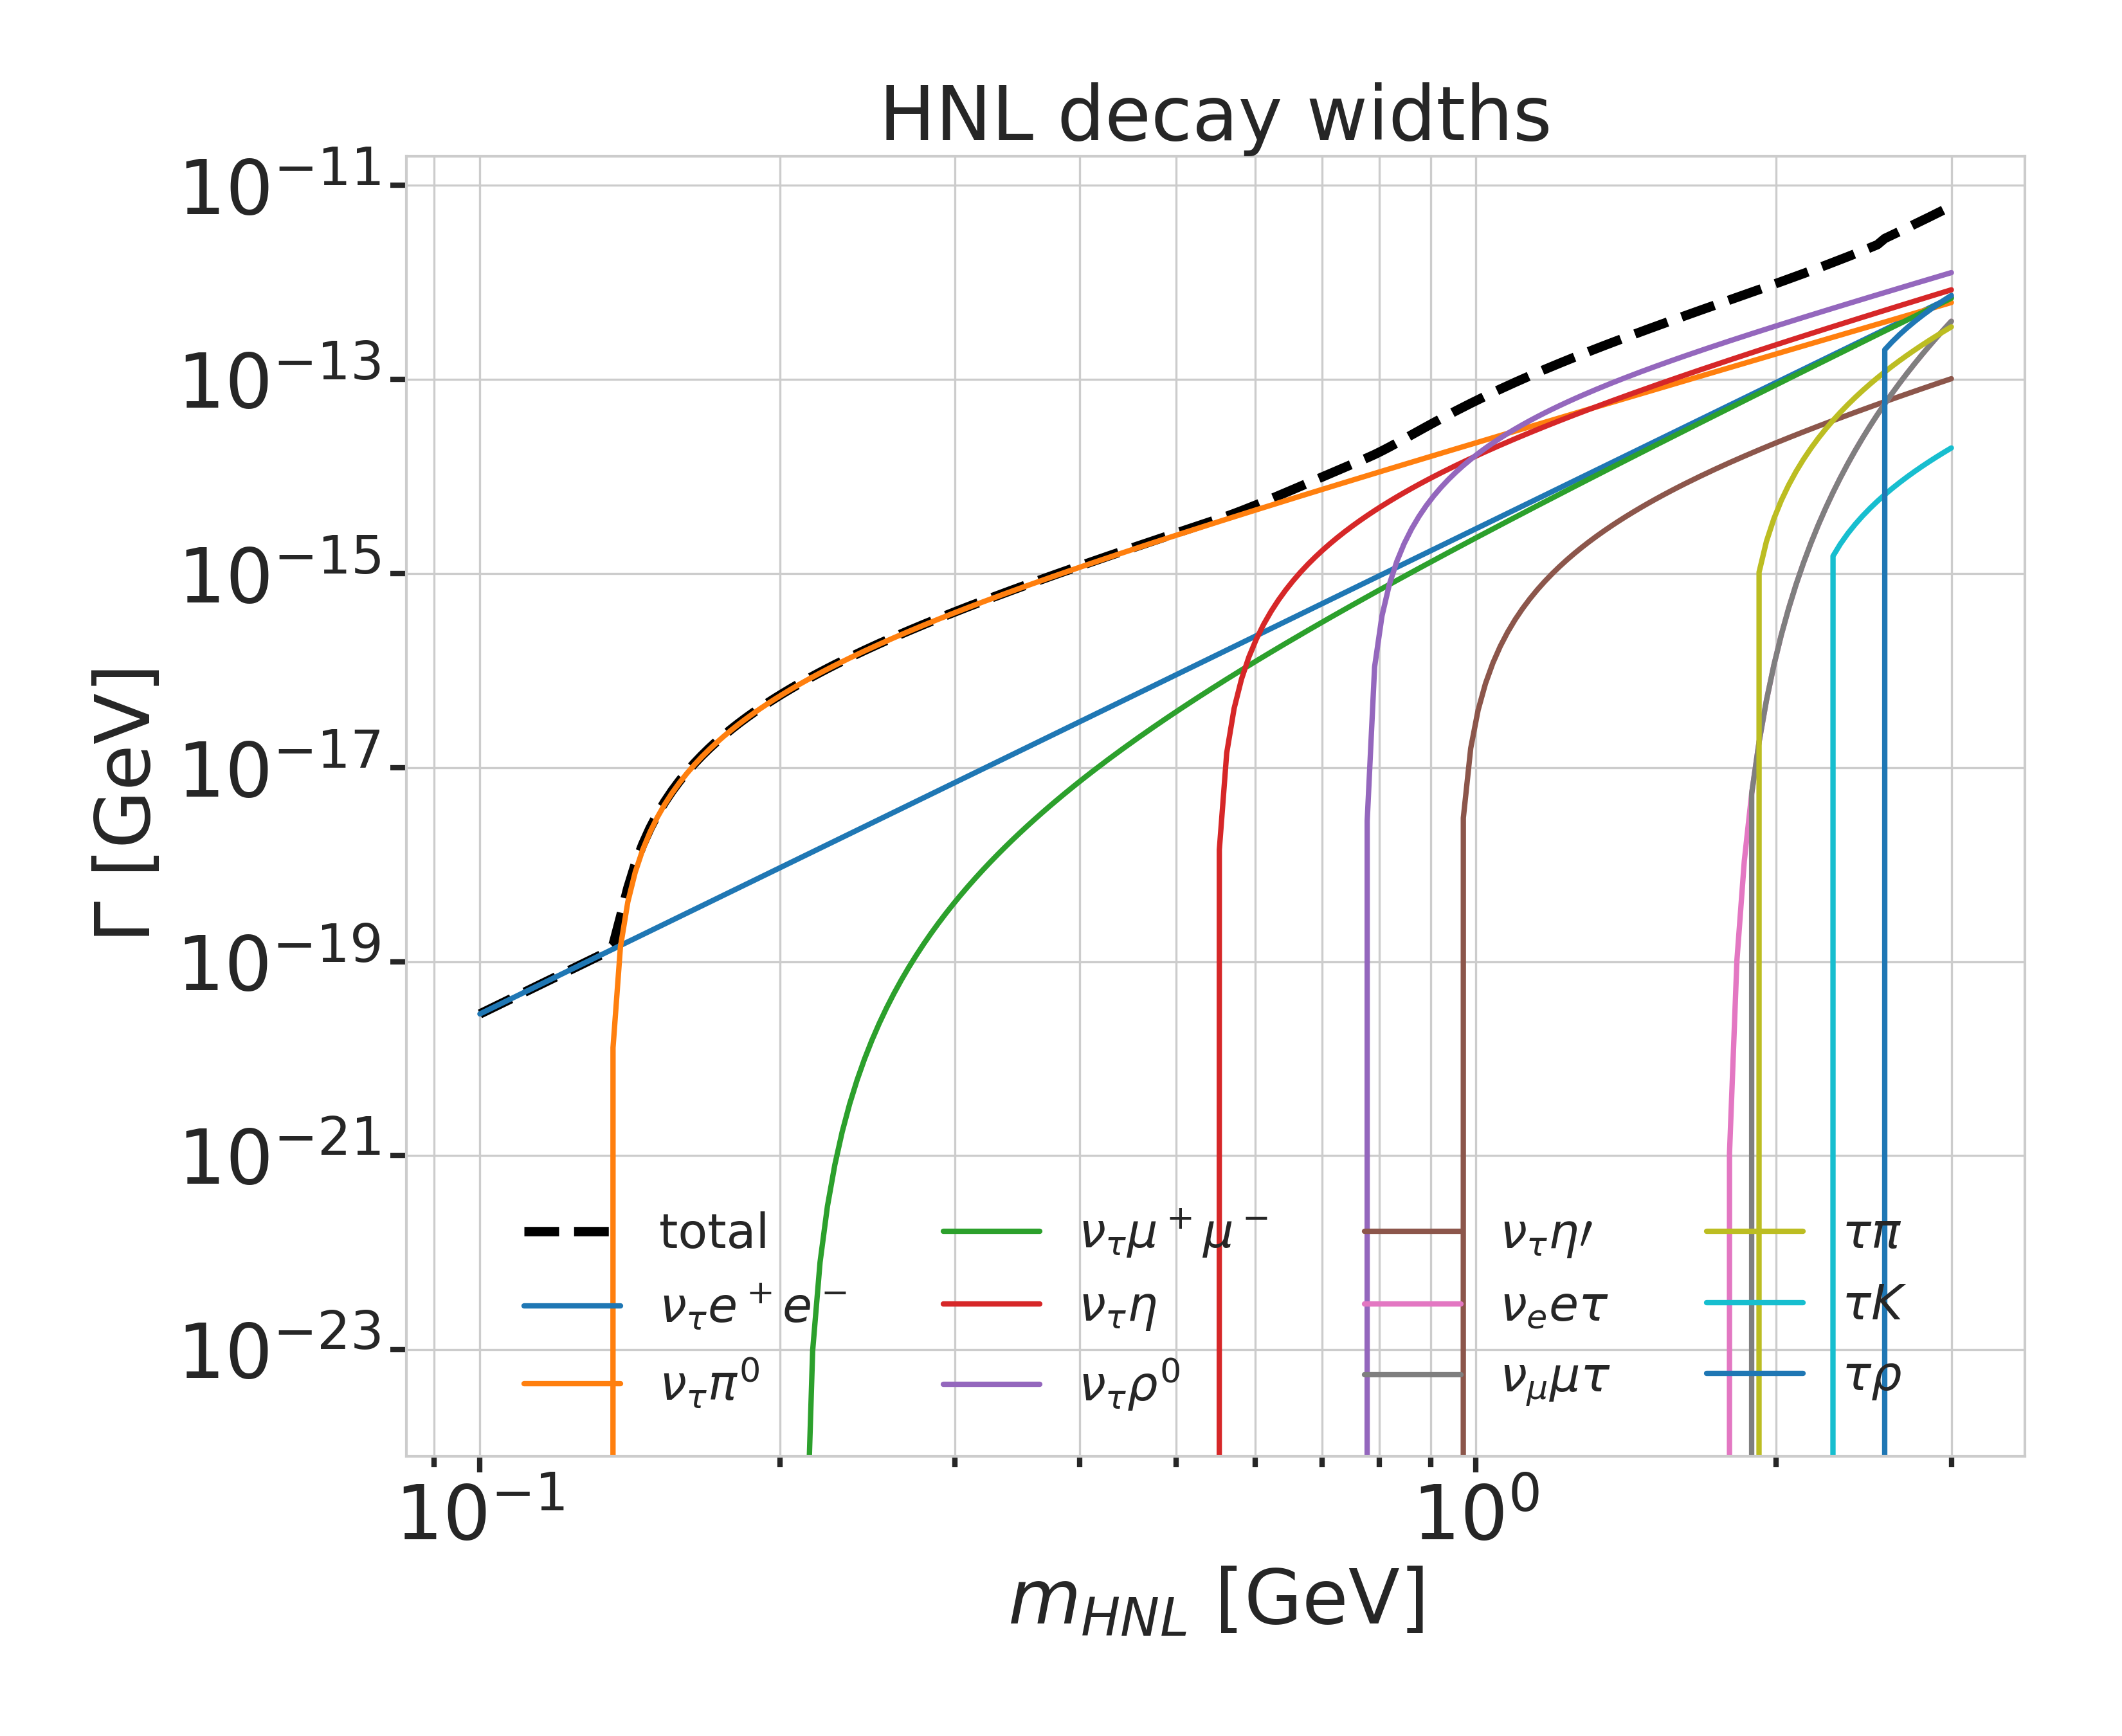
\includegraphics[width=0.7\textwidth]{figures/hnl_decay_widths_log.png}
%   \caption{Decay widths of decay modes visible in IceCube. Calculated based on the results from \cite{Gorbunov:2007ak}.}
%   \label{fig:hnl_visible_decay_widths}
% \end{figure}


\bibliographystyle{JHEP}
\bibliography{MyBibFile}


\end{document}
